\documentclass[../main]{subfiles}

% Appendix B: an appendix adapted from a published paper. An appendix has
% no opening page, so its disclaimer is the appdisclaimer bottom float,
% placed right after the \label. It also shows a figure in an appendix.

\begin{document}
% In a standalone build, switch to appendix numbering and start at B.
\ifSubfilesClassLoaded{\appendix\setcounter{chapter}{1}}{}
\chapter{An adapted appendix}
\label{app:adapted}

\begin{appdisclaimer}
This appendix is adapted from Ref.~\cite{Doe:a26}.
\end{appdisclaimer}

This appendix expands on Chapter~\ref{ch:ch2}.
\lipsum[1][1-5]
In Section~\ref{app:junction} we show a figure.

\section{A junction}
\label{app:junction}
Figure~\ref{fig:mock_appendix} shows the \acrfull{cpr} of a mock junction and its energy levels.
\lipsum[2][1-4]

% No [b] here: on the first page of an appendix the bottom slot belongs to
% the appdisclaimer float, and a figure there would sit below it.
\begin{figure}[htp]
    \centering
    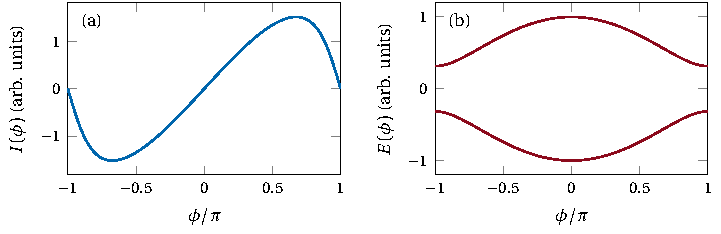
\includegraphics{img/mock_appendix.pdf}
    \caption[A mock-up figure in an appendix]{\textbf{A mock-up figure in an appendix.}
    (a) Mock \acrfull{cpr} of a junction with transmission $\transm = 0.9$.
    (b) The corresponding pair of subgap levels.
    }
    \label{fig:mock_appendix}
\end{figure}

\lipsum[3][1-6]
The \acrshort{cpr} of panel (a) is skewed by the high transmission.

\lipsum[4]

\ifSubfilesClassLoaded{%
\newrefcontext[labelprefix=]
\printbibliography
}{}
\end{document}
